\begin{frame}{Transformer Block}
  \begin{itemize}
    \item[\textcolor{red}{$\blacktriangleright$}] \textbf{Multi-head Attention}
    \item[\textcolor{red}{$\blacktriangleright$}] \textbf{Add \& Norm}
    \item[\textcolor{red}{$\blacktriangleright$}] \textbf{Feed-forward Layer}
    \item[\textcolor{red}{$\blacktriangleright$}] \textbf{Add \& Norm}
  \end{itemize}
  \vspace{1em}
  \textcolor{blue}{\textbf{Note}}\\
  Residual connections and layer normalization are crucial for effective training.
\end{frame}

\begin{frame}{Inside the Transformer Block}
  \begin{itemize}
    \item[\textcolor{red}{$\blacktriangleright$}] The feed-forward sublayer is applied to each position separately, with the same weights at every position:
  \end{itemize}
  \[
    \mathrm{FFN}(x) = \max(0,\, x W_1 + b_1) W_2 + b_2
  \]
  \begin{itemize}
    \item[\textcolor{red}{$\blacktriangleright$}] It widens the representation to $d_{\text{ff}}$ and projects it back, mixing features within a token, whereas attention mixes information across tokens.
    \item[\textcolor{red}{$\blacktriangleright$}] \textbf{Original base model:} 6 encoder blocks and 6 decoder blocks, $d_{\text{model}} = 512$, $h = 8$ heads with $d_k = d_v = 64$, and $d_{\text{ff}} = 2048$.
    \item[\textcolor{red}{$\blacktriangleright$}] At those sizes the feed-forward sublayer holds $2 d_{\text{model}} d_{\text{ff}} \approx 2.1$M weights against $4 d_{\text{model}}^2 \approx 1.0$M for the attention projections: two thirds of the block.
  \end{itemize}
\end{frame}

\begin{frame}{Transformer Block}
  \centering
  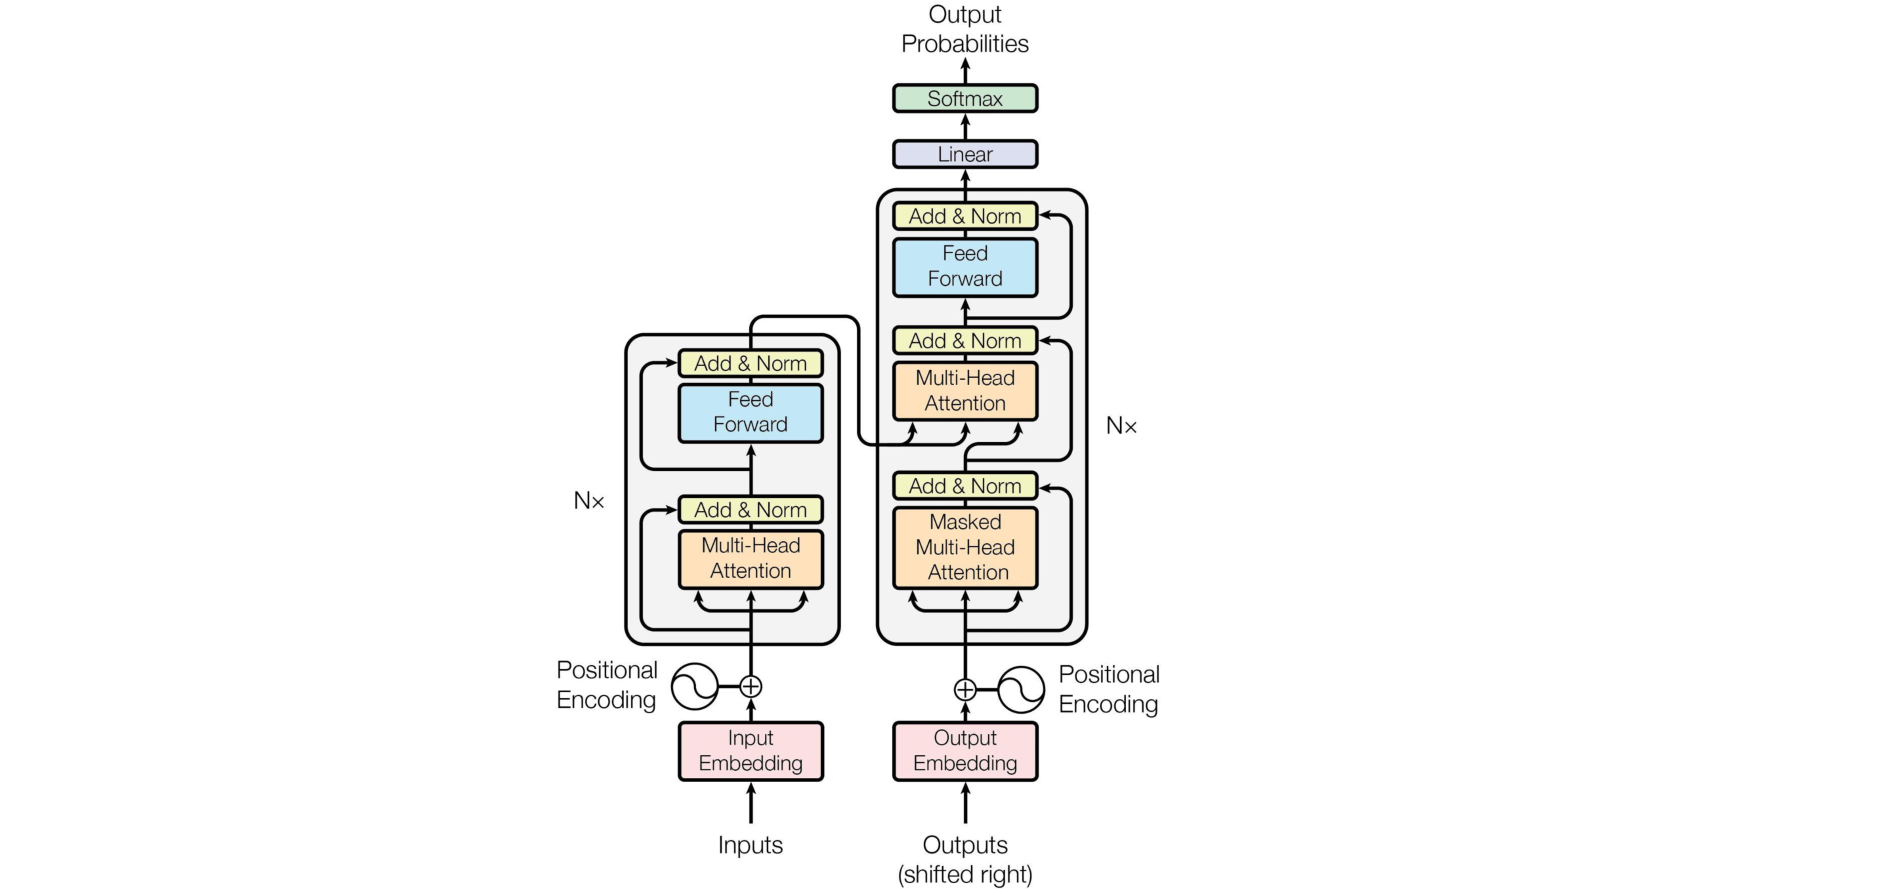
\includegraphics[width=\paperwidth,height=0.71\paperheight,keepaspectratio]{images/introduction-to-transformers/transformer_encoder_decoder_full_architecture.png}

  {\scriptsize Source: Vaswani et al., ``Attention Is All You Need,'' NeurIPS 2017, Fig.~1.}
\end{frame}

